\documentclass[final]{beamer}

% ====================
% Packages
% ====================
\usepackage{fontenc}
\usepackage{lmodern} % Load modern fonts
\usepackage[orientation=portrait,size=a3,scale=1.15]{beamerposter}
\usetheme{gemini}
\usecolortheme{nott}
\usepackage{graphicx}
\usepackage{booktabs}
\usepackage{tikz}
\usepackage{pgfplots}
\usepackage{chemfig}
\usepackage{mhchem}
\pgfplotsset{compat=1.14}
\usepackage{anyfontsize}

% ====================
% Lengths
% ====================
\newlength{\sepwidth}
\newlength{\colwidth}
\setlength{\sepwidth}{0.025\paperwidth}
\setlength{\colwidth}{0.45\paperwidth}

\newcommand{\separatorcolumn}{\begin{column}{\sepwidth}\end{column}}

% ====================
% Title
% ====================
\title{Hvordan fører \text{\textit{Tetraetylbly (\ce{Pb(C_2H_5)_4})}} til kognitiv svekkelse?}
\author{Temor Yari}
\institute[Bjerke Videregående Skole]{Bjerke Videregående Skole}

% ====================
% Footer (optional)
% ====================
\footercontent{1}

% ====================
% Logo (optional)
% ====================
% use this to include logos on the left and/or right side of the header:
% \logoright{\includegraphics[height=2.5cm]{logos/utfpr-logo.png}}
% \logoleft{\hspace{20ex}\includegraphics[height=3.5cm]{logos/ppgca-logo.png}}

% ====================
% Body
% ====================
\begin{document}
\begin{frame}[t]
	\vspace{0.4cm}
	\begin{columns}[t]
		\separatorcolumn

		\begin{column}{\colwidth}

			\begin{block}{Introduksjon}

				\textit{Tetraetylbly (TEL)} ble oppdaget som en effektiv løsning mot motorbanking av
				\textbf{Thomas Midgley Jr.} og \textbf{Charles Kettering} ved General Motors i 1921. Denne
				organometalliske forbindelsen revolusjonerte bilmotorens ytelse ved at den, selv i små
				konsentrasjoner, dramatisk økte bensinens oktantall. TEL under forbrenning danner
				mikroskopiske partikler som fanger frie radikaler og bryter kjedereaksjoner som ellers ville
				ført til Motorbanking.

				\textit{Motorbanking} er et fenomen som oppstår når drivstoff-luft blandingen i motoren
				antennes spontant før tennpluggens gnist. Dette skjer når hydrokarbonmolekylene i bensin med
				lavt oktantall brytes ned under høyt trykk og temperatur tidligere enn ønsket. Resultatet er
				trykkbølger som \textit{banker} mot sylindervegger, noe som både reduserer motorytelsen og
				kan føre til betydelige motorskader over tid.

				I 1924 døde 15 arbeidere grunnen blyforgiftning ved \textbf{Standard Oil's TEL-fabrikk} i
				New Jersey. Til tross for denne tragedien fortsatte bruken i nesten 60 år. På 1970-tallet
				avslørte forsker \textbf{Clair Patterson} sammenhengen mellom TEL og økte blynivåer i
				miljøet og menneskekroppen. Hans arbeid førte til utfasingen av blyholdig bensin som startet
				i USA i 1976 og spredte seg globalt, med dramatisk reduksjon av blynivåer i blodet som
				resultat.

				\begin{figure}[h!]
					\centering
					\vspace{0.5cm}
					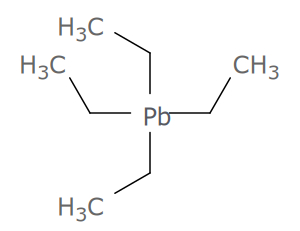
\includegraphics[width=6cm]{./assets/tetraetylblyet.jpg}
					\caption{Tetraetylblyet (\ce{Pb(C_2H_5)})}
				\end{figure}
				\begin{figure}[h!]
					\centering
					\vspace{-0.6cm}
					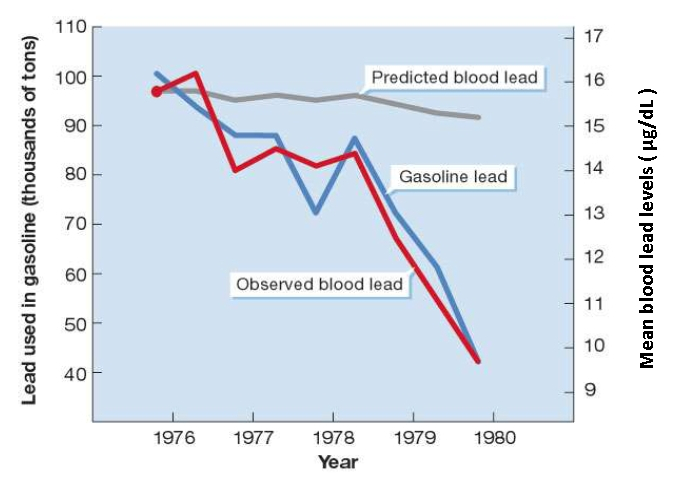
\includegraphics[width=12cm]{./assets/lead_in_gasoline_and_in_blood.jpg}
					\caption{Konsentrasjon av bly (\ce{Pb}) i blod i USA}
				\end{figure}

			\end{block}

			\begin{block}{Teori}
				\textit{Tetraetylbly} (\ce{Pb(C_2H_5)_4}) er en \textbf{organometallisk forbindelse} hvor
				blyatomet er kovalent bundet til fire etylgrupper. Den fungerer som et
				\textit{antikloppmiddel} i bensin ved å øke oktantallet. Under forbrenningen i motoren
				brytes TEL ned til bly og \textit{etylradikaler}$^1$. Disse etylradikaler reagerer da med
				peroksidradikaler som eller ville forårsaket motobanking$^2$. Bly som er igjen fra TEL,
				reagerer med oksygen til \textit{blyoksid}$^3$. For å hindre skadelilg avleiringer tilsettes
				halogenerte forbindelser som reagerer med blyoksidet og danner flyktige
				\textit{blyhalider}$^4$ $^,$ $^5$ som forlater motoren via eksossystemt. Det er oppsumert i
				følgende reaksjosnlininger:

				\begingroup
				\vspace{-0.5cm}
				\Large
				\begin{align}
					\bullet \quad \ce{ & Pb(C2H5)4 -> Pb^{2+} + 4 C2H5^{.}} \\
					\bullet \quad \ce{ & C2H5^{.} + ROO^{.} -> C2H5OOR}     \\
					\bullet \quad \ce{ & Pb + 1/2 O2 -> PbO}                \\
					\bullet \quad \ce{ & PbO + C2H4Br2 -> PbBr2 + C2H4O}    \\
					\bullet \quad \ce{ & PbO + C2H4Cl2 -> PbCl2 + C2H4O}
				\end{align}
				\endgroup
			\end{block}
		\end{column}

		\separatorcolumn

		\begin{column}{\colwidth}
			\vspace{1cm}

			Bly (\ce{Pb}) er et tungmetall med \textbf{høy kjemisk reaktivitet} og kan eksistere i flere
			oksidasjonstilstander, hvorav \ce{Pb^{2+}} er den mest stabile i biologiske systemer. Det har
			en sterk \textbf{affinitet for sulfhydrylgrupper} (\ce{-SH}) i proteiner, noe som betyr at det
			kan lett reagere med enzymer og proteiner som inneholder en eller flere SH-grouper og føre til
			enzymhemming og forstyrrelser i cellulære prosesser. Bly kan også erstatte essensielle
			metaller som \textit{kalsium} (\ce{Ca^{2+}}), \textit{sink} (\ce{Zn^{2+}}) og \textit{jern}
			(\ce{Fe^{2+}/Fe^{3+}}) i proteiner og enzymer, noe som påvirker deres normale fuksjon.

			\vspace{0.5cm}

			\begin{block}{Effekt på menneskets Hjerne}

				\textbf{\delta-Aminolevulinsyre (ALA)} er utgangspunktet for kroppens hemproduksjon. Enzymet
				\textbf{\delta-aminolevulinsyre dehydratase (ALAD)} katalyserer en kondensasjons-reaksjonen
				mellom to ALA-molekyler til \textbf{porfobilinogen (PBG)}. Gjennom flere enzymatiske trinn
				omdannes PBG til \textbf{hem}, den jernholdige komponenten i \textbf{hemoglobin} som er
				avgjørende for \textit{oksygentransport} i blodet.


				\begin{figure}[h!]
					\centering
					\vspace{0.5cm}
					\hspace{-3cm}
					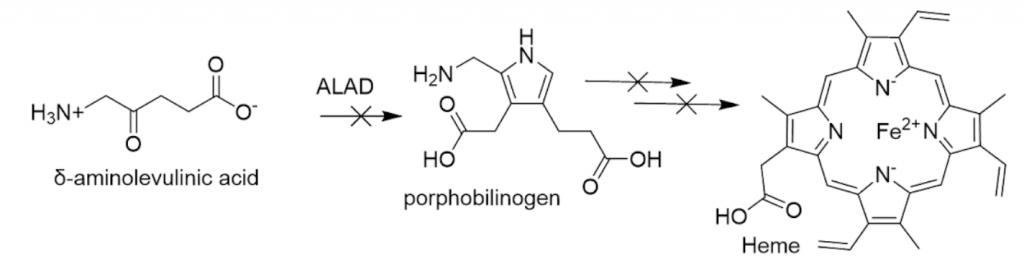
\includegraphics[width=16cm]{./assets/heme_synthesis.png}
					\caption{Hemming av hem-syntese av bly}
				\end{figure}
				\vspace{0.2cm}

				Bly utøver sin toksiske effekt ved å erstatte \textit{sink} (\ce{Zn^{2+}}) i ALADs
				metallbindingssete, noe som hemmer enzymets aktivitet. Dette resulterer i to skadelige
				effekter: \textbf{redusert PBG- og hemproduksjon} som fører til \textbf{nedsatt
					oksygentransport}, samt akkumulering av ALA. Overskudd av ALA er særlig skadelig fordi det
				kan krysse \textbf{blod-hjerne-barrieren} og generere reaktive oksygenforbindelser
				(\ce{ROS}) i hjernen. ROS er kjemisk reaktive molekyler som \textit{superoksidanion}
				(\ce{O_2^{-.}}), \textit{hydrogenperoksid} (\ce{H_2O_2}) og \textit{hydroksylradikal}
				(\ce{OH^{.}}), som dannes når ALA gjennomgår auto-oksidasjon og redoksreaksjoner.

				\begin{figure}[h!]
					\centering
					\vspace{0.5cm}
					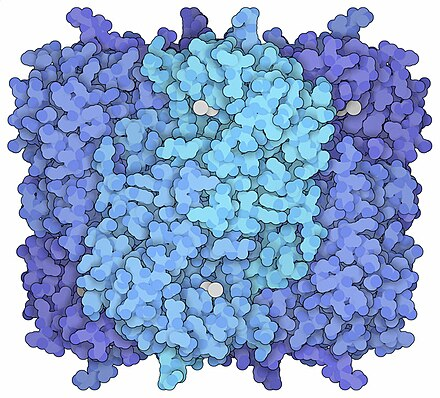
\includegraphics[width=12cm]{./assets/ALAD_poisoned_by_lead_ions.jpg}
					\caption{ALAD-enzymet forgiftet av bly}
				\end{figure}
				\vspace{0.5cm}

				\textbf{Calmodulin} og \textbf{proteinkinase C (PKC)} er to annen viktige \textit{kalsium
					styrte proteiner} i cellene som blir påvirket av bly. Calmodulin fungerer som en
				\textit{av/på-bryter} når kalsium binder seg til det, og hjelper til med å sende signaler
				mellom nerveceller. PKC er en gruppe enzymer som også aktiveres av kalsium og hjelper celler
				med å dele seg og utvikle seg. Bly kan erstatte kalsiumet i begge disse proteinene fordi de
				ligner i størrelse og ladning. Dette fører til: med calmodulin får vi en bryter som sitter
				fast i \textit{på}-posisjonen, mens PKC blir blokkert og slutter å virke når det er mye bly
				til stede.

			\end{block}
		\end{column}

		\separatorcolumn

	\end{columns}
\end{frame}
\end{document}
